\section{Skaitiniai modeliai}

\subsection{Erdvės diskretizavimas}

Abiems skaitiniams modeliams naudosime tokiu pačiu principu sukonstruotą tinklelį. Jį sudarydami padaliname stačiakampę erdvę $\Omega$ į $N\times M$ taškų, kurie yra nutolę vienas nuo kito fiksuotais atstumais $\Delta x$ ir $\Delta y$ atitinkamomis ašimis. Analogiškai, laiko erdvę $[0, T]$ padalinsime į $\tau + 1$ taškų, kurie vienas nuo kito yra nutolę tolygiais $\Delta t$ atstumais. Apibūdinta diskretų tinklelį galima užrašyti taip:

\begin{align}
    \omega_W&=\{ x_i : x_i = i\Delta x, \quad i=0, 1, \dots, N - 1 \} & \Delta x&=\frac{W}{N-1} \label{meshx}\\
    \omega_H&=\{ y_j : y_j = j\Delta y, \quad j=0, 1, \dots, M - 1 \} & \Delta y&=\frac{H}{M-1} \label{meshy}\\
    \omega_\tau&=\{ t_n : t_n = n\Delta t,\quad n=0, 1, \dots, \tau\} & \Delta t&=\frac{T}{\tau} \label{mesht}\\
	\omega&=\omega_W\times\omega_H\times\omega_\tau \label{mesh}
\end{align}

\begin{figure}[!h]
\centering
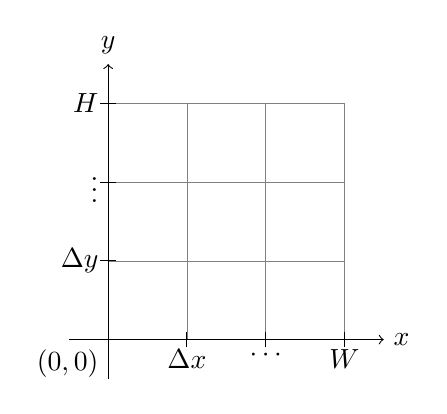
\begin{tikzpicture}
    
% Define the size of the cells
\def\Deltax{1} % Delta x size
\def\Deltay{1} % Delta y size
\def\Xmax{4} % Max X value
\def\Ymax{4} % Max Y value

% Draw the mesh
\foreach \x in {0,1,2} {
    \foreach \y in {0,1,2} {
        \draw[help lines] (\x*\Deltax,\y*\Deltay) grid (\x*\Deltax+\Deltax,\y*\Deltay+\Deltay);
    }
}

\node[below left] at (0,0) {$(0, 0)$};

% Draw axes
\draw[->] (-0.5,0) -- (3.5 *\Deltax,0) node[right] {$x$} ;
\draw[->] (0,-0.5) -- (0,3.5) node[above] {$y$};

% Add tick marks on x-axis with labels
\draw[shift={(1,0)}] (0,-0.1) -- (0,0.1);
\node[below] at (1, 0) {\(\Delta x\)};

\draw[shift={(2,0)}] (0,-0.1) -- (0,0.1);
\node[below] at (2, 0) {$\cdots$};

\draw[shift={(3,0)}] (0,-0.1) -- (0,0.1);
\node[below] at (3, 0) {$W$};

% Add tick marks on y-axis with labels

\draw[shift={(0,1)}] (-0.1,0) -- (0.1,0);
\node[left] at (0, 1) {$\Delta y$};
        
\draw[shift={(0,2)}] (-0.1,0) -- (0.1,0);
\node[left] at (0, 2) {$\vdots$};

\draw[shift={(0,3)}] (-0.1,0) -- (0.1,0);
\node[left] at (0, 3) {$H$};

\end{tikzpicture}
\caption{ Diskretizuota erdvė }
\end{figure}

\newpage

\subsection{Išreikštinis FTCS metodas}

Remiantis išreikštiniu FTCS (\textit{angl. forward time centered space}) metodu pakeisime sistemos \eqref{rect} lygtis su išvestinių aproksimacijomis gautomis skleidžiant išvestines pagal Teiloro eilutę.

\begin{subequations} \label{finite-diffs}
\begin{align}
	\frac{\partial c}{\partial t}\Big|_{x=x_i, y=y_j, t=t_n}&=\frac{c^{n+1}_{i,j}-c^n_{i,j}}{\Delta t} + \mathcal{O}(\Delta t)\\
    \frac{\partial^2c}{\partial x^2}\Big|_{x=x_i, y=y_j, t=t_n}&=\frac{c^n_{i-1,j} - 2c^n_{i,j} + c^n_{i+1,j}}{(\Delta x)^2} + \mathcal{O}((\Delta x)^2)\\
    \frac{\partial^2c}{\partial y^2}\Big|_{x=x_i, y=y_j, t=t_n}&=\frac{c^n_{i,j-1} - 2c^n_{i,j} + c^n_{i,j+1}}{(\Delta y)^2} + \mathcal{O}((\Delta y)^2)
\end{align}
\end{subequations}

Įstate aproksimacijų išraiškas gauname dvimatį skaitini modelį:

\begin{subequations} \label{numerical-eqs}
	\begin{align}
		\frac{c^{n+1}_{1,i,j}-c^n_{1,i,j}}{\Delta t} & =
		-3kc^{n}_{1,i,j}c^{n}_{2,i,j}\notag\\
        & +D\left(\frac{c^n_{1,i-1,j}-2c^n_{1,i,j}+c^n_{1,i+1,j}}{(\Delta x)^2}+\frac{c^n_{1,i,j-1}-2c^n_{1,i,j}+c^n_{1,i,j+1}}{(\Delta y)^2}\right) \\
		\frac{c^{n+1}_{2,i,j}-c^n_{2,i,j}}{\Delta t} & =
		-5kc^{n}_{1,i,j}c^{n}_{2,i,j}\notag\\
        &+D\left(\frac{c^n_{2,i-1,j}-2c^n_{2,i,j}+c^n_{2,i+1,j}}{(\Delta x)^2}+\frac{c^n_{2,i,j-1}-2c^n_{2,i,j}+c^n_{2,i,j+1}}{(\Delta y)^2}\right) \\
		\frac{c^{n+1}_{3,i,j}-c^n_{3,i,j}}{\Delta t} & =2kc^{n}_{1,i,j}c^{n}_{2,i,j},
	\end{align}
\end{subequations}

Čia
$\Delta t$ - laiko žingsnis,
$\Delta x$ - diskrečios erdvės žingsnis $x$ ašimi,
$\Delta y$ - diskrečios erdvės žingsnis $y$ ašimi.
$c^n_{1,i,j}$, $c^n_{2,i,j}$, $c^n_{3,i,j}$ - atitinkamai pirmos, antros ir trečios medžiagų koncentracijos diskretizuotos erdvės tinklelio taške $(x_i, y_i, t_n)\in\omega$.

\subsection{Neišreikštinis kintamos krypties metodas}

% Ka galima butu rasyti apie sita metoda
% kontekstas, is kur jis, kam skiras, pliusai ir minusai

Neišreikštinį kintamos krypties metodą (\textit{alternating direction implicit, ADI}) JAV mokslininkai Donald W. Peaceman ir Henry H. Rachford Jr. pristatė savo straipsnyje \enquote{skaitinis sprendinys parabolinėms ir elipsinės diferencialinėms lygtims}. Nuo to laiko šis metodas plačiai taikomas matematinio modeliavimo srityje. Kaip galima suprasti iš straipsnio pavadinimo, šis metodas pritaikytas spręsti parabolines ir elipsines diferencialinių lygčių sistemas, ypatingai tada, kai sistema turi daugiau nei vieną erdvinę dimensiją. Kadangi mūsų nagrinėjamą sistemą sudaro parabolinės diferencialinės lygtys jį ir taikysime.

Šis metodas yra tarpinis variantas tarp Išreikštinio FTCS ir Crank-Nicholson metodo, kuriuo bandoma išlaikyti sprendimo greitį, tačiau taip pat ir tikslumą. Įprastoms parabolinėms lygtims šis metodas būna besąlygiškai stabilus \cite{liAlternatingDirectionImplicit2021}, tai leidžia pasirinkti bet kokio dydžio laiko žingsnį ir tokiu būdu sumažinti bendrą laiko žingsnių kiekį, kurį reikia įvykdyti. Toliau pritaikysime metodą nagrinėjamai sistemai.

Tarkime turime skaitinį sprendinį konkrečių laiko momentu $t^n$, kaip ir anksčiau, jį žymėsime $c^n$. Vietoje to, kad tiesiogiai skaičiuotume skaitinį sprendinį sekančiu laiko momentu $c^{n + 1}$, apskaičiuosime tarpinį sprendinį, kurį žymėsime $c^*$. Šis sprendinys ypatingas tuo, kad jo ieškodami $x$ dimensiją laikysime išreikštine, o $y$ dimensiją -- neišreikštine:

\begin{align}
    \frac{c^* - c^n}{\frac{1}{2}\Delta t} = ...
\end{align}

